\section{Wprowadzenie}

\subsection{Cel dokumentu}
Celem dokumentu jest zdefiniowanie wymagań dla czatu ViuaChat na podstawie analizy otoczenia aplikacji oraz analizy potrzeb projektu w stosunku do niej.

\subsection{Zakres dokumentu}
Niniejszy dokument jest produktem pierwszego etapu procesu wytwórczego czatu ViuaChat, na który składają się:
\begin{itemize}
    \item analiza otoczenia, wraz z z klientami;
    \item wskazanie kontekstu biznesowego systemu;
    \item określenie udziałowców;
	\item wyszczególnienie i uporządkowanie zasad biznesowych, jakie zostały założone w stosunku do aplikacji;
	\item opracowanie historyjek na podstawie ustalonych zasad biznesowych.
\end{itemize}

\textbf{Uwaga:} Niniejszy dokument nie dotyczy języka ViuAct ani jego kompilatora.

Praca wygenerowana w systemie \LaTeX.

\subsection{Dokumenty powiązane}
\begin{itemize}
	\item Szkic funkcjonalności ViuaChat - pierwszy zarys zasad biznesowych, ujęty w formie prostego konspektu;
	\item Specyfikacja wymagań biznesowych i \textit{user stories} - starsza wersja dokumentu SWS, nieujmująca otoczenia i kontekstu aplikacji.
\end{itemize}

\subsection{Odbiorcy}
Dokument został skierowany przede wszystkim dla członków zespołu, aby ułatwić im współpracę - w szczególności wówczas, gdy funkcjonalności czatu mogą pociągać za sobą modyfikację zestawu bibliotek ViuaVM bądź struktury składni projektowanego języka ViuAct.

Kolejną grupą adresatów niniejszego dokumentu są pracownicy uczelni, odpowiedzialni za nadzór nad prawidłowym ukształtowaniem i przebiegiem projektu. Wśród nich, szczególną rolę odgrywa JE Dziekan ZWI, prof. Marek Bednarczyk, będący opiekunem projektu.

\subsection{Słownik pojęć}
\begin{description}
  \item[Pokój] Współdzielony czat, do którego dostęp ma równocześnie wielu uczestników, widzących nawzajem wysyłane przez siebie wiadomości
  \item[Wpięcie użytkownika w pokój] Rodzaj relacji, polegający na tym, że dany użytkownik ma możliwość nadawania i odbierania wiadomości w ramach określonego pokoju
  \item[Wiadomości prywatne] Wiadomości, które są wysyłane konkretnemu użytkownikowi i są widoczne wyłącznie dla nadawcy i odbiorcy takiej wiadomości
  \item[ViuAct] Język programowania wysokiego poziomu, oparty o model aktorów, powstały na potrzeby niniejszego projektu inżynierskiego
\end{description}

\section{Czat w kontekście}

\subsection{Kontekst biznesowy}

Niniejszy czat stanowi część szerszego kontekstu, jakim jest potrzeba zademonstrowania działania języka ViuAct oraz całego środowiska wytwórczego powiązanego z maszyną wirtualną ViuaVM.

\begin{figure}[h]
	\centering
	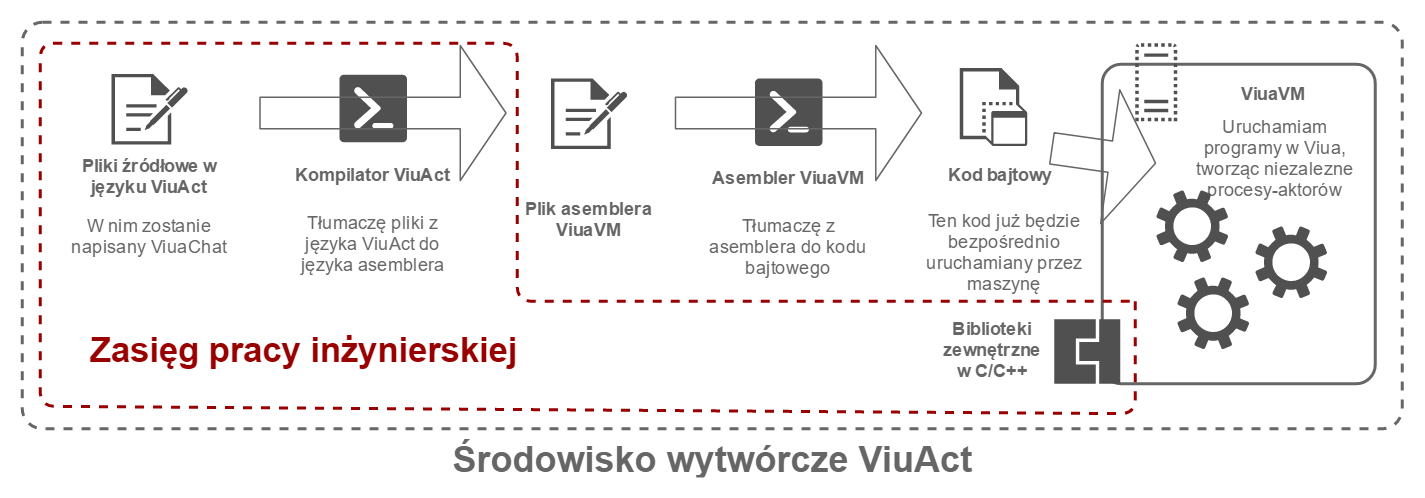
\includegraphics[width=\textwidth]{chat/fig/viuavm-env}
	\caption{Ilustracja środowiska wytwórczego wraz zasięgiem, którym są objęte prace przewidziane projektem inżynierskim}
\end{figure}

Cel demonstracyjny jest pierwszym i najważniejszym, jaki przyświeca konstrukcji czatu. Ponadto, sam proces wytwórczy pozwoli
przetestować wydajność całego środowiska w jego praktycznym wymiarze. Tym samym, możliwe będzie poprawienie konstrukcji kompilatora 
lub zastosowanych konstrukcji językowych ViuAct, podnoszących jego użyteczność.

Wszelcy odbiorcy dla aplikacji czatu zostaną, podobnie jak sama aplikacja, skonstruowani na cele demonstracyjne. Nie powinni oni
odbiegać od modelowych odbiorców podobnych komunikatorów, tak, aby potencjalny, poczatkujący użytkownik środowiska ViuaVM mógł
zrozumieć intencje stojące za rozwiązaniami zastosowanymi w ViuaChat oraz przenieść je do swoich pierwszych programów, opracowanych
w tym środowisku.

\subsection{Udziałowcy}

Poniżej wyszczególniono udziałowców, mających wpływ na rozwój czatu.

\begin{tabular}{ | l | l | }
  
	\hline
	\multicolumn{2}{ | l | }{\textbf{Karta udziałowca}}  \\
  
	\hline
    \parbox[t]{3cm}{
    	\textbf{Identyfikator}
    } & UN-01 \\  
    
    \hline
    \parbox[t]{3cm}{
    	\textbf{Nazwa}
    } & ViuaVM \\  
    
    \hline
    \parbox[t]{3cm}{
    	\textbf{Opis}
    } & \parbox[t]{12cm}{
    	Maszyna wirtualna, oparta o przechowywanie danych w rejestrach zamiast \textit{płaskich} tablic pamięci. Stanowi ona 
    	platformę, na której musi zostać uruchomiony serwer czatu. Ponieważ jej największym atutem jest zorientowanie na kod
    	wykonywany współbieżnie, sam serwer czatu powinien tę cechę wykorzystywać w maksymalnym stopniu. 
    	} \\ 
    
    \hline
    \parbox[t]{3cm}{
    	\textbf{Typ}
    } & Nieożywiony, bezpośredni \\  
    
    \hline
    \parbox[t]{3cm}{
    	\textbf{Punkt widzenia}
    } & \parbox[t]{12cm}{
    	ViuaVM jest absolutnie nieodzownym elementem projektu, a serwer czatu stanowi przede wszystkim dowód jej użyteczności.
    	O ile jądro maszyny nie ma być poddawane już żadnym zmianom i być wykorzystane takie, jakie było na inicjalnym etapie
    	pracy inżynierskiej, o tyle dopuszcza się poszerzanie jej funkcjonalności o dodatkowe biblioteki zewnętrzne.
    	} \\ 
    
    \hline
    \parbox[t]{3cm}{
    	\textbf{Ograniczenia}
    } & \parbox[t]{12cm}{
    	Maszyna wirtualna, jakkolwiek stanowi istotny czynnik dla decyzji w zakresie architektury czy konstrukcji oprogramowania,
    	nie powinna mieć wpływu na wymagania stricte biznesowe, jest bowiem jedynie środowiskiem do uruchamiania współbieżnych
    	programów, \textit{przezroczystym} dla końcowego użytkownika czy zleceniodawcy zrealizowanego oprogramowania.
    	} \\ 
    
    \hline
    \parbox[t]{3cm}{
    	\textbf{Wymagania}
    } & \colorbox{yellow}{...} \\ 
  
    \hline
\end{tabular}

\vspace{2em} 

\begin{tabular}{ | l | l | }

	\hline
	\multicolumn{2}{ | l | }{\textbf{Karta udziałowca}}  \\
  
	\hline
    \parbox[t]{3cm}{
    	\textbf{Identyfikator}
    } & UO-01 \\  
    
    \hline
    \parbox[t]{3cm}{
    	\textbf{Nazwa}
    } & Opiekun pracy inżynierskiej \\ 
    
    \hline
    \parbox[t]{3cm}{
    	\textbf{Opis}
    } & \parbox[t]{12cm}{
    	Pracownik uczelni, wyznaczony do opieki nad całym projektem inżynierskim - nadzorowania jego postępów, wskazywania problemów
    	oraz sugerowania decyzji podwyższających walor pracy oraz szanse na jej skuteczne obronienie. Ma również zasadniczy wpływ na 
    	decyzję o dopuszczeniu pracy do recenzji.
    } \\ 
    
    \hline
    \parbox[t]{3cm}{
    	\textbf{Typ}
    } & Ożywiony, bezpośredni \\  
    
    \hline
    \parbox[t]{3cm}{
    	\textbf{Punkt widzenia}
    } & \parbox[t]{12cm}{
    	Opiekun pracy patrzy na czat przede wszystkim przez pryzmat jego użyteczności jako efektownego przykładu implementacji modelu
    	aktora w praktycznym, programistycznym ujęciu. Stąd, jego uwaga skupia się przede wszystkim na konstrukcjach językowych,
    	strukturach oraz rozwiązaniach od strony kodu źródłowego. Czat stanowi jedynie pretekst do przeniesienia teoretycznych, akademickich
    	rozważań na praktyczny grunt. 
    	} \\ 
    
    \hline
    \parbox[t]{3cm}{
    	\textbf{Ograniczenia}
    } & \parbox[t]{12cm}{
    	Opiekun pracy, pomimo bycia jej nadzorcą i posiadania istotnych uprawnień decyzyjnych w stosunku do jej dalszego rozwoju, 
    	nie ma możliwości bieżącego śledzenia prac oraz
    	podejmowania decyzji w przypadku konkretnych problemów. Powinien zachować dystans, pozwalający na samodzielną realizację projektu
    	przez zespół. Stąd, jego faktyczny udział ogranicza się do udzielania porad w przypadku strategicznych kierunków, w jakich
    	będzie podążała grupa, a także doraźnego recenzowania ograniczonej puli zagadnień, wyłapanych w trakcie wspólnych spotkań.
    	} \\ 
    
    \hline
    \parbox[t]{3cm}{
    	\textbf{Wymagania}
    } & \colorbox{yellow}{...} \\ 
  
    \hline
\end{tabular}

\vspace{2em} 

\begin{tabular}{ | l | l | }

	\hline
	\multicolumn{2}{ | l | }{\textbf{Karta udziałowca}}  \\
  
	\hline
    \parbox[t]{3cm}{
    	\textbf{Identyfikator}
    } & UO-02 \\  
    
    \hline
    \parbox[t]{3cm}{
    	\textbf{Nazwa}
    } & \parbox[t]{12cm}{
    Członek zespołu ds. ViuAct
    } \\ 
    
    \hline
    \parbox[t]{3cm}{
    	\textbf{Opis}
    } & \parbox[t]{12cm}{
    	Student i członek zespołu, skupiający się w pierwszej kolejności nad rozwojem języka programowania ViuAct, jego kompilatora oraz
    	ewentualnego rozbudowania maszyny ViuaVM o kolejne, zewnętrzne biblioteki.
    } \\ 
    
    \hline
    \parbox[t]{3cm}{
    	\textbf{Typ}
    } & Ożywiony, bezpośredni \\  
    
    \hline
    \parbox[t]{3cm}{
    	\textbf{Punkt widzenia}
    } & \parbox[t]{12cm}{
    	Przede wszystkim, postrzega czat jako produkt, realizowany na końcowej platformie. Stąd, musi brać udział w formułowaniu
    	wymagań związanych z ViuaVM oraz językiem ViuAct. Jego zadaniem jest doprowadzenia do zaprojektowania czatu w sposób, 
    	który ukaże możliwości ViuAct jako solidnego, kompletnego rozwiązania. Przy tym, musi trzymać rękę na pulsie i reagować,
    	gdyby pojawiały się przeszkody w zaprogramowaniu czatu, wynikające z niedoskonałości środowiska wytwórczego.
    	
    	Podczas współudziału w definiowaniu wymagań, istotny jest dla niego zakres pracy, wiążący się z 
    	urzeczywistnianiem poszczególnych, proponowanych wymagań. Zbyt rozbudowany czat może opóźnić prace nad całym projektem,
    	a w efekcie - zniweczyć trud włożony w rozwój języka programowania i dedykowanego mu kompilatora.
    	} \\ 
    
    \hline
    \parbox[t]{3cm}{
    	\textbf{Ograniczenia}
    } & \parbox[t]{12cm}{
    	Jego udział w pracach nad czatem jest z gruntu nieograniczony. Jednakże, decydując się na podział odpowiedzialności 
    	podyktowany zespołowym charakterem projektu oraz własnymi ograniczeniami czasowymi, zrezygnował z decydowania o biznesowej 
    	części wymagań, faktycznie pozostając w roli konsultanta.
    	
    	} \\ 
    
    \hline
    \parbox[t]{3cm}{
    	\textbf{Wymagania}
    } & \colorbox{yellow}{...} \\ 
  
    \hline
\end{tabular}

\vspace{2em} 

\begin{tabular}{ | l | l | }

	\hline
	\multicolumn{2}{ | l | }{\textbf{Karta udziałowca}}  \\
  
	\hline
    \parbox[t]{3cm}{
    	\textbf{Identyfikator}
    } & UO-03 \\  
    
    \hline
    \parbox[t]{3cm}{
    	\textbf{Nazwa}
    } & \parbox[t]{12cm}{
    Członek zespołu ds. Czatu
    } \\ 
    
    \hline
    \parbox[t]{3cm}{
    	\textbf{Opis}
    } & \parbox[t]{12cm}{
    	Student i członek zespołu, odpowiedzialny za prace nad czatem
    } \\ 
    
    \hline
    \parbox[t]{3cm}{
    	\textbf{Typ}
    } & Ożywiony, bezpośredni \\  
    
    \hline
    \parbox[t]{3cm}{
    	\textbf{Punkt widzenia}
    } & \parbox[t]{12cm}{
    	Czat stanowi dla niego, obok dokumentacji, najistotniejszą część przedsięwzięcia. Musi z jednej strony nauczyć się poruszać
    	w nowym, dynamicznie zmieniającym się środowisku programistycznym, a z drugiej strony - zrealizować przy jego użyciu serwer
    	czatu, który pokaże jego możliwości i zastosowania innym nowicjuszom.
    	
    	Podczas współudziału w definiowaniu wymagań, istotny jest dla niego zakres końcowych funkcjonalności czatu. Nie może być zbyt 
    	wąski. Z drugiej strony, konstrukcja programu powinna pozostać prosta i przejrzysta. Przykładowy kod nie powinien odstraszać
    	potencjalnego programisty, dla którego cała koncepcja ViuaVM oraz modelu aktorów może wydawać się na pierwszy rzut oka nieco egzotyczna.
    	} \\ 
    
    \hline
    \parbox[t]{3cm}{
    	\textbf{Ograniczenia}
    } & \parbox[t]{12cm}{
    	Nie ma w zasadzie organizacyjnych czy kompetencyjnych ograniczeń dla formułowania wymagań. Nie oznacza to jednak, że może
    	definiować wymagań w oderwaniu od pozostałych udziałowców (ich role i punkty widzenia opisano wcześniej).
    	} \\ 
    
    \hline
    \parbox[t]{3cm}{
    	\textbf{Wymagania}
    } & \colorbox{yellow}{...} \\ 
  
    \hline
\end{tabular}

\subsection{Charakterystyka użytkowników}

Na etapie analizy kontekstu, w którym ma zostać zaprojektowany i zrealizowany czat, zadecydowano o zaprojektowaniu następujących,
modelowych użytkowników docelowego oprogramowania:

\begin{enumerate}

	\item \textbf{Użytkownik tymczasowy.} Typ użytkownika, którego konto jest tworzone podczas połączenia z serwerem czatu oraz 
		niszczone po jego zakończeniu. Podczas łączenia z czatem, nie będzie musiał się autoryzować przy użyciu hasła, a deklarować
		tylko unikalną nazwę, nie powtarzającą się z nazwą innego użytkownika, posiadającego konto na danym serwerze czatu. Ten typ
		konta jest przeznaczony dla osób, zainteresowanych dołączeniem do dyskusji na czacie bez dodatkowych zobowiązań.
		
	\item \textbf{Użytkownik stały.} Typ użytkownika, którego konto jest utrzymywane przez serwer pomiędzy połączeniami do czatu. W
		zamierzeniu, adresatami takiego rozwiązania mają być stali bywalcy serwera, którzy chcą mieć zarezerwowaną określoną nazwę
		dla siebie i uniknąć ewentualnego podszywania się. Stąd każdorazowo, przed rozpoczęciem sesji połączenia z serwerem, muszą się
		dodatkowo autoryzować przy użyciu hasła. Równocześnie, ich nazwa jest zarezerwowana wyłącznie do jego użytku oraz niedostępna
		dla użytkowników tymczasowych.
		
	\item \textbf{Administrator.} To użytkownik stały, który jest dodatkowo wyróżniony i posiada uprawienia do szeroko pojętego 
		zarządzania serwerem (w tym - pozostałymi użytkownikami). Nie wyróżnia się wśród administratorów żadnych dodatkowych, szczególnych
		ról (np. superadministrator, właściciel).
		
\end{enumerate}

Poza wspomnianymi różnicami, wszyscy użytkownicy po rozpoczęciu sesji połączenia mają prawo do dołączania do pokojów oraz wysyłania sobie
nawzajem wiadomości prywatnych. Łącznie, pula użytkowników przebywających na serwerze czatu w jednym momencie nie powinna przekraczać 320,
zaś w jednym pokoju - nie więcej niż 32. W związku z tym można przyjąć, że czat jest przeznaczony dla niewielkich społeczności, np.
szkolnych, uczelnianych czy hobbystycznych.

\subsection{Istniejąca infrastruktura}

\begin{itemize}
	\item \textbf{Komputer A}
	\begin{itemize}
		\item komputer przenośny z procesorem Intel Core i5 oraz systemem operacyjnym Windows 10
		\item XAMPP 7.2.7, obejmujący serwer Apache 2.4 oraz interpreter języka PHP w wersji 7.2.7.
	\end{itemize}
	
	\item \textbf{Komputer B}
	\begin{itemize}
		\item komputer przenośny, na którym zainstalowano system operacyjny Linux Mint 19 ,,Tara''
		\item GNU Compiler Collection 8.2
		\item wirtualna maszyna Viua VM w wersji 0.9.0
		\item \textit{należy doinstalować serwer Nginx, odpowiedzialny za wysłanie frontendu do
		użytkownika łączącego się z czatem oraz za handshake Websocketu}
	\end{itemize}
	
	\item \textit{\textbf{Do uzupełnienia}
	\begin{itemize}
		\item Kolejne urządzenie końcowe (trzecie), dzięki któremu będzie można symulować połączenie kolejnej
		osoby do usługi czatu
	\end{itemize}}

\end{itemize}

\section{Zasady biznesowe}

Zidentyfikowane zasady pogrupowano w 3 kategorie, biorąc pod uwagę podstawowe bloki funkcjonalności. Przydzielenie
do kategorii jest sygnalizowanie literą alfabetu, będącą prefiksem identyfikatora danej zasady. Dokonano
również priorytetyzacji zasad biznesowych według klasycznej skali ,,MoSCoW":

\begin{itemize}
	\item \textbf{,,M''} (z ang. \textit{must}) - zasady, których spełnienie jest niezbędne dla realizacji systemu
	\item \textbf{,,S''} (z ang. \textit{should}) - są to zasady o wysokim priorytecie, które powinny;
	zostać spełnione, o ile tylko jest to możliwe;
	\item \textbf{,,C''} (z ang. \textit{could}) - dobrze byłoby zrealizować takie wymagania, ale zależy to od czasu
	i zasobów, jakie pozostaną do dyspozycji po ukończeniu zadań ,,M" i ,,C";
	\item \textbf{,,W''} (z ang. \textit{won't}) - takie wymagania, po dyskusji, zostały wycofane dalszej realizacji.
\end{itemize}

\subsection{System użytkowników [ZU]}
  \begin{tabular}{ | l | l | l | }
	\hline
    \textbf{ID} & \parbox[t]{14cm}{
    	\textbf{Zasada biznesowa}
    } & \textbf{Priorytet} \\  
  
    \hline
    ZU-01 & \parbox[t]{14cm}{
      Podczas wejścia na czat, użytkownikowi pokazuje się monit z polem do wpisania nazwy użytkownika. 
    } & M \\

    \hline
    ZU-02 & \parbox[t]{14cm}{
      Użytkownicy bez stałego konta podczas logowania podają tylko nazwę użytkownika, pole hasła pozostaje puste .
    } & M \\

    \hline
    ZU-03 & \parbox[t]{14cm}{
      Nazwa użytkownika to ciąg od 3 do 32 alfanumerycznych znaków.
    } & M \\

    \hline
    ZU-04 & \parbox[t]{14cm}{
      Można rozpocząć sesję jako użytkownik, pod warunkiem, że zadeklarowana nazwa nie będzie powtarzać się z nazwami już zalogowanych użytkowników. 
    } & M \\

    \hline
    ZU-05 & \parbox[t]{14cm}{
      Monit podczas wejścia na czat jest wyposażony w pole do wpisania hasła (nieobowiązkowe). 
    } & S \\

    \hline
    ZU-06 & \parbox[t]{14cm}{
      Użytkownicy czatu ze stałym kontem, podczas logowania podają nazwę i odpowiadające mu hasło.
    } & S \\

    \hline
    ZU-07 & \parbox[t]{14cm}{
      Stałe konta użytkowników są utrzymywane na serwerze w postaci trójek wartości: nazwa użytkownika, hasło (md5), czy jest administratorem. 
    } & S \\

    \hline
    ZU-08 & \parbox[t]{14cm}{
      Nie można rozpocząć sesji użytkownika o nazwie, która pasuje do istniejącego konta, jeżeli nie zostanie podane prawidłowe hasło (nie można podszywać się pod nazwy użytkowników ze stałym kontem).
    } & S \\

    \hline
    ZU-09 & \parbox[t]{14cm}{
      Można rozpocząć sesję jako użytkownik bez podawania hasła, pod warunkiem, że zadeklarowana nazwa nie będzie powtarzać się z nazwami stałych kont użytkowników.
    } & S \\

    \hline
    ZU-10 & \parbox[t]{14cm}{
      W okienkach czatu, loginy użytkowników ze stałym kontem są pogrubione i pokolorowane: Administratorzy na czerwono,
      Pozostali na zielono. 
      } & S \\

    \hline
    ZU-11 & \parbox[t]{14cm}{
      Administratorzy mają prawo przeglądać nazwy pokojów na serwerze. 
    } & M \\

    \hline
    ZU-12 & \parbox[t]{14cm}{
      Administratorzy mają prawo tworzyć i usuwać pokoje. 
    } & S \\

    \hline
    ZU-13 & \parbox[t]{14cm}{
      Administratorzy mają prawo ustanawiać, zmieniać i usuwać hasła do pokojów. 
    } & C \\

    \hline
    ZU-14 & \parbox[t]{14cm}{
      Administratorzy mają prawo wyrzucać użytkowników z pokojów. 
    } & C \\

    \hline
    ZU-15 & \parbox[t]{14cm}{
      Administratorzy mają prawo wyrzucać użytkowników z serwera. 
    } & C \\

    \hline
    ZU-16 & \parbox[t]{14cm}{
      Administratorzy mają prawo przeglądać nazwy i poziomy uprawnień kont stałych użytkowników. 
    } & M \\

    \hline
    ZU-17 & \parbox[t]{14cm}{
      Administratorzy mają prawo tworzyć i usuwać użytkowników. 
    } & S \\

    \hline
    ZU-18 & \parbox[t]{14cm}{
      Administratorzy mają prawo zmieniać hasła użytkowników. 
    } & C \\

    \hline
    ZU-19 & \parbox[t]{14cm}{
      Administratorzy mają prawo zmieniać uprawnienia stałych kont użytkowników. 
    } & C \\

    \hline
    ZU-20 & \parbox[t]{14cm}{
      Użytkownicy ze stałymi kontami mogą zmieniać swoje hasło.
    } & W \\

    
    \hline
  \end{tabular}

\subsection{Pokoje [ZP]}
  \begin{tabular}{ | l | l | l | }
	\hline
    \textbf{ID} & \parbox[t]{14cm}{
    	\textbf{Zasada biznesowa}
    } & \textbf{Priorytet} \\  
    
    \hline
    ZP-01 & \parbox[t]{14cm}{
      Pokoje to właściwe czaty – tam użytkownicy mogą wejść i pisać do siebie nazwajem
    } & M \\

    \hline
    ZP-02 & \parbox[t]{14cm}{
      Każdy pokój ma unikalną nazwę będącą ciągiem alfanumerycznym od 3 do 32 znaków
    } & M \\

    \hline
    ZP-03 & \parbox[t]{14cm}{
      Lista pokojów jest widoczna dla każdego użytkownika po zalogowaniu się do serwera czatu
    } & M \\

    \hline
    ZP-04 & \parbox[t]{14cm}{
      Użytkownik może być równocześnie wpięty do jednego pokoju
    } & M \\

    \hline
    ZP-05 & \parbox[t]{14cm}{
      Wiadomość wysłana w pokoju jest widoczna w oknie pokoju dla wszystkich użytkowników podpiętych do tego pokoju
    } & M \\

    \hline
    ZP-06 & \parbox[t]{14cm}{
      Użytkownik może się samodzielnie wypiąć z pokoju, do którego jest wpięty
    } & S \\

    \hline
    ZP-07 & \parbox[t]{14cm}{
      Pokój może mieć ustanowione hasło, które użytkownik musi wpisać przed podpięciem się do niego
    } & C \\
    
    \hline
    ZP-08 & \parbox[t]{14cm}{
      Nowo wpięty użytkownik widzi 10 najnowszych wiadomości, 
      które zostały wysłane do pokoju tuż przed wpięciem
    } & S \\
    
    \hline
    ZP-09 & \parbox[t]{14cm}{
      Serwer czatu automatycznie wysyła do pokoju wiadomości, 
      zawierające powiadomienia o wydarzeniach związanych z
      pokojem, tzw. wiadomości systemowe
    } & S \\
    
    \hline
    ZP-10 & \parbox[t]{14cm}{
      Wiadomości systemowe są niepodpisane przez
      żadnego użytkownika i zapisane kursywą
   	} & C \\
   	
   	\hline
    ZP-11 & \parbox[t]{14cm}{
      Wiadomość systemowa zostaje wysłana podczas wpięcia się
      nowego użytkownika do pokoju
   	} & S \\
   	
   	\hline
    ZP-12 & \parbox[t]{14cm}{
      Wiadomość systemowa zostaje wysłana podczas wypięcia
      użytkownika z pokoju
   	} & S \\
   	
   	\hline
    ZP-13 & \parbox[t]{14cm}{
      Wiadomość systemowa zostaje wysłana, gdy użytkownik
      wpięty do pokoju traci połączenie z serwerem czatu
   	} & S \\
   	
   	\hline
    ZP-14 & \parbox[t]{14cm}{
      Wiadomość systemowa zostaje wysłana, gdy użytkownik
      zostaje wyrzucony z pokoju
   	} & S \\	
    
    \hline
    
  \end{tabular}

\subsection{Prywatne wiadomości [ZW]}
  \begin{tabular}{ | l | l | l | }
  	\hline
    \textbf{ID} & \parbox[t]{14cm}{
    	\textbf{Zasada biznesowa}
    } & \textbf{Priorytet} \\  
    
    \hline
    ZW-01 & \parbox[t]{14cm}{
      Wiadomości prywatne to wiadomości, które są wysyłane do
      konkretnego odbiorcy, innego niż nadawca. Są one widoczne
      wyłącznie dla nadawcy i odbiorcy takiej wiadomości
    } & M \\

    \hline
    ZW-02 & \parbox[t]{14cm}{
      Wiadomość prywatna może być wysłana z okna czatu pokoju – wiadomości prywatne nie są pokazywane wszystkim uczestnikom czatu, a jedynie użytkownikowi, do którego jest adresowana. 
    } & M \\

    \hline
    ZW-03 & \parbox[t]{14cm}{
      Aby wysłać wiadomość prywatną w oknie pokoju, należy poprzedzić ją znakiem \# i nazwą użytkownika, do którego jest kierowana wiadomość, oddzielona spacją od komunikatu, np.: „\#user Tajna wiadomość”.
    } & C \\

    \hline
    ZW-04 & \parbox[t]{14cm}{
      W oknie czatu pokoju dopuszczalne jest wysyłanie wiadomości prywatnych tylko tych użytkowników, którzy są do niego w danym momencie podpięci
    } & C \\

    \hline
    ZW-05 & \parbox[t]{14cm}{
      Próba wysłania wiadomości prywatnej w pokoju powinna zostać
      odrzucona przez serwer i zwrócić błąd w przypadku gdy:
      \begin{itemize}
      	\item Po znaku „\#” pojawi się od razu znak spacji lub nie
      	będzie żadnych znaków (nie zostanie podana 
		nazwa użytkownika który jest adresatem)
		\item Nazwa adresata jest dłuższa niż 32 znaki
		\item Wysyłamy wiadomość prywatną w pokoju czatu do
		użytkownika, który nie jest podpięty do tego pokoju
      \end{itemize}
		
    } & M \\
    
    \hline
    ZW-06 & \parbox[t]{14cm}{
      Użytkownik dysponuje dedykowanym oknem, w którym widzi wiadomości prywatne. 
    } & M \\
    
    \hline
    ZW-07 & \parbox[t]{14cm}{
      Z okna wiadomości prywatnych można odbierać i wysyłać wyłącznie
      wiadomości prywatne, których nadawcą/odbiorcą jest wybrany
      użytkownik
    } & M \\    
    
    \hline
    ZW-08 & \parbox[t]{14cm}{
      W oknie wiadomości prywatnych można przeglądać wiadomości wysłane do i odebrane od jednego, wybranego użytkownika.
      
    } & S \\
    
    \hline
    ZW-09 & \parbox[t]{14cm}{
      W oknie wiadomości prywatnych można wysyłać wiadomości
      wyłącznie do nadawcy, którego wiadomości są w danym momencie
      pokazywane.
    } & S \\
    
    \hline
    ZW-10 & \parbox[t]{14cm}{
      Czas istnienia wiadomości prywatnych zależy od typu użytkownika
      który jest jej nadawcą i odbiorcą:
      \begin{itemize}
      	\item Jeżeli co najmniej jedna strona komunikacji
      	 jest użytkownikiem tymczasowym, wiadomości są
      	 utrzymywane dopóki nadawca i odbiorca nie skończą
      	 sesji na serwerze
      	\item Jeżeli jedna strona komunikacji jest
      	użytkownikiem
      	tymczasowym, a druga stałym, to wiadomość jest utrzymywana
      	dopóki użytkownik tymczasowy skończy sesję połączenia z
      	serwerem
      	\item Jeżeli obie strony są użytkownikami stałymi, to
      	wiadomość jest trzymana bezterminowo
      \end{itemize}
    } & S \\
    
    \hline
    ZW-11 & \parbox[t]{14cm}{
      Dla każdej pary użytkowników, na serwerze jest
      gromadzone co najwyżej 100 wiadomości prywatnych.
    } & S \\
    \hline
  \end{tabular}

\section{Wymagania}

\subsection{Wymagania funkcjonalne}

Ponieważ obraną metodologią wytwarzania aplikacji jest \textit{mini-Scrum}, należący do kategorii metodyk zwinnych, wymagania funkcjonalne ujęto w formie historyjek (\textit{user stories}).

\vspace{2em} 

\begin{tabular}{ | l | l | }
	\hline
		\textbf{Identyfikator} & 
		WF-01
		\\
		
	\hline
		\textbf{Treść} & \parbox[t]{11cm}{
			Jako użytkownik serwera czatu, chcę się do niego zalogować, aby zobaczyć listę pokojów dyskusyjnych.
		}\\
		 
	\hline
		\parbox[t]{4cm}{\textbf{Powiązane zasady biznesowe}} & \parbox[t]{11cm}{
			ZU-01 Podczas wejścia na czat, użytkownikowi pokazuje się monit z polem do wpisania nazwy użytkownika. \\
			ZP-03 Lista pokojów jest widoczna dla każdego użytkownika
			po zalogowaniu się do serwera czatu
		}\\
		
	\hline
		\parbox[t]{4cm}{\textbf{Kryteria akceptacji}} & \parbox[t]{11cm}{
			\begin{enumreq}
				\item Po wejściu na czat bez rozpoczętej sesji, pokazuje się monit o podanie nazwy użytkownika.
				\item Po wpisaniu nazwy użytkownika i zatwierdzeniu, użytkownik rozpocznie sesję na serwerze czatu.
				\item Tuż po rozpoczęciu sesji czatu, użytkownik zobaczy listę pokojów.
			\end{enumreq}
			}
		\\

	\hline
\end{tabular}

\vspace{2em} 

\begin{tabular}{ | l | l | }
	\hline
		\textbf{Identyfikator} & 
		WF-02
		\\
		
	\hline
		\textbf{Treść} & \parbox[t]{11cm}{
			Jako użytkownik serwera czatu, chcę wpiąć się do pokoju,
			aby wziąć udział w dyskusji.
		}\\
		 
	\hline
		\parbox[t]{4cm}{\textbf{Powiązane zasady biznesowe}} & \parbox[t]{11cm}{
			ZP-01 Pokoje to właściwe czaty - tam użytkownicy mogą
			wejść i pisać do siebie nawzajem
		}\\
		
	\hline
		\parbox[t]{4cm}{\textbf{Kryteria akceptacji}} & \parbox[t]{11cm}{
			\begin{enumreq}
				\item Użytkownik, który ma otwartą sesję 
				połączenia z serwerem czatu i nie jest wpięty
				do żadnego pokoju, zobaczy listę pokojów.
				\item Użytkownik, po kilknięciu w liście pokojów
				na nazwę pokoju, zostanie do niego podpięty
				\item Użytkownik po wpięciu się do pokoju zobaczy
				okno pokoju
				\item Użytkownik, który ma otwartą sesję
				połączenia z serwerem i jest wpięty do pokoju,
				po odświeżeniu przeglądarki zobaczy okno pokoju, 
				do którego jest wpięty
			\end{enumreq}
			}
		\\

	\hline
\end{tabular}

\vspace{2em} 

\begin{tabular}{ | l | l | }
	\hline
		\textbf{Identyfikator} & 
		WF-03
		\\
		
	\hline
		\textbf{Treść} & \parbox[t]{11cm}{
			Jako użytkownik serwera czatu, chcę po wpięciu
			do pokoju zobaczyć ostatnie wiadomości wysłane
			przed moim dołączeniem, aby dowiedzieć się, co
			tam się obecnie dzieje.
		}\\
		 
	\hline
		\parbox[t]{4cm}{\textbf{Powiązane zasady biznesowe}} & \parbox[t]{11cm}{
			ZP-08 Nowo wpięty użytkownik widzi 10 najnowszych
			wiadomości, które zostały wysłane do pokoju tuż
			przed wpięciem
		}\\
		
	\hline
		\parbox[t]{4cm}{\textbf{Kryteria akceptacji}} & \parbox[t]{11cm}{
			\begin{enumreq}
				\item Użytkownik po wpięciu się do pokoju zobaczy
				10 najnowszych wiadomości wysłanych do pokoju
				przed jego dołączeniem (lub mniej, jeżeli
				dotychczas nie wysłano do pokoju co najmniej
				10 wiadomości)
			\end{enumreq}
			}
		\\

	\hline
\end{tabular}

\vspace{2em} 

\begin{tabular}{ | l | l | }
	\hline
		\textbf{Identyfikator} & 
		WF-04
		\\
		
	\hline
		\textbf{Treść} & \parbox[t]{11cm}{
			Jako użytkownik serwera czatu, chcę chcę wysłać
			wiadomość do pokoju w który jestem wpięty, aby
			zobaczyli ją inni uczestnicy dyskusji.
		}\\
		 
	\hline
		\parbox[t]{4cm}{\textbf{Powiązane zasady biznesowe}} & \parbox[t]{11cm}{
			ZP-01 Pokoje to właściwe czaty - tam użytkownicy mogą
			wejść i pisać do siebie nawzajem
		}\\
		
	\hline
		\parbox[t]{4cm}{\textbf{Kryteria akceptacji}} & \parbox[t]{11cm}{
			\begin{enumreq}
				\item Użytkownik wpisze tekst wiadomości w polu
				tekstowym u dołu czatu
				\item Wiadomość wpisana w polu tekstowym zostanie
				wysłana po wciśnięciu klawisza ,,Enter'', gdy aktywne
				będzie pole tekstowe
				\item Wiadomość wpisana w polu tekstowym zostanie
				wysłana po naciśnięciu przycisku ,,Wyślij'',
				widocznego obok pola tekstowego
				\item Po wysłaniu wiadomości, pole tekstowe zostanie
				wyczyszczone (niezależnie od tego czy wiadomość
				zostanie doręczona)
				\item Wiadomość wysłana do pokoju jest pokazywana
				wszystkim użytkownikom podpiętym do czatu u dołu
				strony
				\item Nowa wiadomość jest pokazywana wraz z nazwą
				użytkownika wysyłającego u dołu konwersacji
			\end{enumreq}
			}
		\\

	\hline
\end{tabular}

\vspace{2em} 

\begin{tabular}{ | l | l | }
	\hline
		\textbf{Identyfikator} & 
		WF-05
		\\
		
	\hline
		\textbf{Treść} & \parbox[t]{11cm}{
			Jako użytkownik serwera czatu, chcę chcę zobaczyć
			powiadomienie o wpięciu się nowego użytkownika do
			pokoju w którym sam jestem obecnie wpięty, aby powitać
			nowego dyskutanta
		}\\
		 
	\hline
		\parbox[t]{4cm}{\textbf{Powiązane zasady biznesowe}} & \parbox[t]{11cm}{
			ZP-09 Serwer czatu automatycznie wysyła do pokoju
			wiadomości, zawierające powiadomienia o wydarzeniach
			związanych z pokojem, tzw. wiadomości systemowe \\
			ZP-11 Wiadomość systemowa zostaje wysłana podczas
			wpięcia się nowego użytkownika do pokoju
		}\\
		
	\hline
		\parbox[t]{4cm}{\textbf{Kryteria akceptacji}} & \parbox[t]{11cm}{
			\begin{enumreq}
				\item Niezwłocznie po wpięciu się użytkownika do
				pokoju, serwer wyśle wiadomość systemową o treści
				,,Użytkownik ... dołączył do pokoju'', widoczną
				dla wszystkich użytkowników wpiętych do tego pokoju
			\end{enumreq}
			}
		\\

	\hline
\end{tabular}

\vspace{2em} 

\begin{tabular}{ | l | l | }
	\hline
		\textbf{Identyfikator} & 
		WF-06
		\\
		
	\hline
		\textbf{Treść} & \parbox[t]{11cm}{
			Jako użytkownik serwera czatu, chcę zobaczyć
			powiadomienie o opuszczeniu pokoju przez użytkownika,
			aby łatwo zorientować się, że nie bierze już udziału 
			w dyskusji.
		}\\
		 
	\hline
		\parbox[t]{4cm}{\textbf{Powiązane zasady biznesowe}} & \parbox[t]{11cm}{
			ZP-09 Serwer czatu automatycznie wysyła do pokoju
			wiadomości, zawierające powiadomienia o wydarzeniach
			związanych z pokojem, tzw. wiadomości systemowe \\
			ZP-12 Wiadomość systemowa zostaje wysłana podczas
			wpięcia wypięcia użytkownika z pokoju \\
			ZP-13 Wiadomość systemowa zostaje wysłana, gdy użytkownik
			wpięty do pokoju traci połączenie z serwerem \\
			ZP-14 Wiadomość systemowa zostaje wysłana, gdy użytkownik
			zostaje wyrzucony z pokoju
			
		}\\
		
	\hline
		\parbox[t]{4cm}{\textbf{Kryteria akceptacji}} & \parbox[t]{11cm}{
			\begin{enumreq}
				\item Niezwłocznie po wypięciu się użytkownika z
				pokoju, serwer wyśle wiadomość systemową, widoczną
				dla wszystkich użytkowników wpiętych do tego pokoju,
				o treści:
				\begin{enumerate}
					\item ,,Użytkownik ... opuścił pokój'', gdy
					użytkownik samodzielnie wypiął się z pokoju
					\item ,,Użytkownik ... stracił połączenie'',
					gdy użytkownik został wypięty z pokoju na skutek
					przerwania sesji z uwagi na zerwanie połączenia
					\item ,,Użytkownik ... został wyrzucony'', gdy
					użytkownik został wypięty wskutek interwencji
					administratora
				\end{enumerate}
			\end{enumreq}
			}
		\\

	\hline
\end{tabular}

\vspace{2em} 

\begin{tabular}{ | l | l | }
	\hline
		\textbf{Identyfikator} & 
		WF-07
		\\
		
	\hline
		\textbf{Treść} & \parbox[t]{11cm}{
			Jako użytkownik serwera czatu, chcę odpiąć się od pokoju,
			aby wpiąć się do innego pokoju.
		}\\
		 
	\hline
		\parbox[t]{4cm}{\textbf{Powiązane zasady biznesowe}} & \parbox[t]{11cm}{
			ZP-06 Użytkownik może się samodzielnie wypiąć z pokoju,
			do którego jest wpięty
			
		}\\
		
	\hline
		\parbox[t]{4cm}{\textbf{Kryteria akceptacji}} & \parbox[t]{11cm}{
			\begin{enumreq}
				\item W oknie pokoju użytkownik zobaczy przycisk
				lub link ,,Opuść pokój''.
				\item Po kliknięciu w ,,Opuść pokój'', użytkownik
				zobaczy listę pokojów.
			\end{enumreq}
			}
		\\

	\hline
\end{tabular}

\vspace{2em} 

\begin{tabular}{ | l | l | }
	\hline
		\textbf{Identyfikator} & 
		WF-08
		\\
		
	\hline
		\textbf{Treść} & \parbox[t]{11cm}{
			Jako użytkownik serwera czatu, chcę zobaczyć
			okno wiadomości prywatnych, aby odczytać wiadomości,
			które wysłano specjalnie do mnie.
		}\\
		 
	\hline
		\parbox[t]{4cm}{\textbf{Powiązane zasady biznesowe}} & \parbox[t]{11cm}{
			ZW-01 Wiadomości prywatne to wiadomości, które są
			wysyłane do konkretnego odbiorcy, innego niż
			nadawca... \\
			ZW-06 Użytkownik dysponuje dodatkowym oknem, na którym
			widzi wiadomości prywatne. \\
			ZW-07 Z okna wiadomości prywatnych można odbierać i
			wysyłać wyłącznie wiadomości prywatne, których
			nadawcą / odbiorcą jest wybrany użytkownik. \\
		}\\
		
	\hline
		\parbox[t]{4cm}{\textbf{Kryteria akceptacji}} & \parbox[t]{11cm}{
			\begin{enumreq}
				\item Po kliknięciu w link ,,PW'', użytkownik
				zobaczy okno prywatnych wiadomości
				\item W oknie wiadomości prywatnych, użytkownik
				zobaczy listę użytkowników, od których otrzymał
				wiadomości prywatne.
				\item Po kliknięciu w link z nazwą użytkownika,
				użytkownik zobaczy prywatne wiadomości, których
				nadawcą i odbiorcą jest wskazana osoba.
			\end{enumreq}
			}
		\\

	\hline
\end{tabular}

\vspace{2em} 

\begin{tabular}{ | l | l | }
	\hline
		\textbf{Identyfikator} & 
		WF-09
		\\
		
	\hline
		\textbf{Treść} & \parbox[t]{11cm}{
			Jako użytkownik serwera czatu, chcę wysłać
			wiadomość prywatną do jednego użytkownika, aby
			prowadzić z nim ciągłą konwersację.
		}\\
		 
	\hline
		\parbox[t]{4cm}{\textbf{Powiązane zasady biznesowe}} & \parbox[t]{11cm}{
			
			
		}\\
		
	\hline
		\parbox[t]{4cm}{\textbf{Kryteria akceptacji}} & \parbox[t]{11cm}{
			\begin{enumreq}
				\item Użytkownik wpisze tekst wiadomości w polu
				tekstowym u dołu okna wiadomości prywatnych
				\item Wiadomość wpisana w polu tekstowym zostanie
				wysłana po wciśnięciu klawisza ,,Enter'', gdy
				aktywne
				będzie pole tekstowe
				\item Wiadomość wpisana w polu tekstowym zostanie
				wysłana po naciśnięciu przycisku ,,Wyślij'',
				widocznego obok pola tekstowego
				\item Po wysłaniu wiadomości, pole tekstowe zostanie
				wyczyszczone (niezależnie od tego czy wiadomość
				zostanie doręczona)
				\item Wiadomość wysłana w oknie zostanie pokazana
				tylko użytkownikowi, z którym trwa otwarta
				konwersacja
				\item Nowa wiadomość jest pokazywana wraz z nazwą
				użytkownika wysyłającego u dołu konwersacji
			\end{enumreq}`								
			}
		\\

	\hline
\end{tabular}


\vspace{2em} 

\begin{tabular}{ | l | l | }
	\hline
		\textbf{Identyfikator} & 
		WF-10
		\\
		
	\hline
		\textbf{Treść} & \parbox[t]{11cm}{
			Jako użbytkownik czatu, chcę wysłać wiadomość
			prywatną w oknie czatu, aby zobaczył ją tylko jej
			odbiorca
		}\\
		 
	\hline
		\parbox[t]{4cm}{\textbf{Powiązane zasady biznesowe}} & \parbox[t]{11cm}{
			
			
		}\\
		
	\hline
		\parbox[t]{4cm}{\textbf{Kryteria akceptacji}} & \parbox[t]{11cm}{
			\begin{enumreq}
				\item Użytkownik wpisze w oknie pokoju 
				wiadomość zapoczątkowaną znakiem kratki \# i nazwą 
				użytkownika obecnego na czacie, oddzieloną spacją 
				od treści wiadomości
				tekstowym u dołu okna wiadomości prywatnych
				\item Wiadomość wysłana w oknie zostanie pokazana
				tylko użytkownikowi, do którego została skierowana
				a także u tego użytkownika, który ją nadał
				\item Wiadomości prywatna w oknie pokoju jest
				podświetlona na żółto.
			\end{enumreq}`								
			}
		\\

	\hline
\end{tabular}


\vspace{2em} 

\begin{tabular}{ | l | l | }
	\hline
		\textbf{Identyfikator} & 
		WF-11
		\\
		
	\hline
		\textbf{Treść} & \parbox[t]{11cm}{
			Jako użytkownik serwera czatu, chcę wysłać wiadomość 
			prywatną do innego użytkownika, z którym wcześniej nie
			wymieniałem takich wiadomości, aby rozpocząć z nim
			prywatną konwersację.
		}\\
		 
	\hline
		\parbox[t]{4cm}{\textbf{Powiązane zasady biznesowe}} & \parbox[t]{11cm}{
			
			
		}\\
		
	\hline
		\parbox[t]{4cm}{\textbf{Kryteria akceptacji}} & \parbox[t]{11cm}{
			\begin{enumreq}
				\item Użytkownik kliknie w oknie wiadomości
				prywatnych w przyciski ,,Nowy''.
				\item Użytkownik zobaczy monit o podanie nazwy
				użytkownika, z którym chce rozpocząć rozmowę
				\item Jeżeli użytkownik jest aktywny, wówczas 
				\item Wiadomość wpisana w polu tekstowym zostanie
				wysłana po wciśnięciu klawisza ,,Enter'', gdy
				aktywne
				będzie pole tekstowe
				\item Wiadomość wpisana w polu tekstowym zostanie
				wysłana po naciśnięciu przycisku ,,Wyślij'',
				widocznego obok pola tekstowego
				\item Po wysłaniu wiadomości, pole tekstowe zostanie
				wyczyszczone (niezależnie od tego czy wiadomość
				zostanie doręczona)
				\item Wiadomość wysłana w oknie zostanie pokazana
				tylko użytkownikowi, z którym trwa otwarta
				konwersacja
				\item Nowa wiadomość jest pokazywana wraz z nazwą
				użytkownika wysyłającego u dołu konwersacji
			\end{enumreq}`								
			}
		\\

	\hline
\end{tabular}

\subsection{Wymagania niefunkcjonalne}

\begin{tabular}{ | l | l | }
	\hline
		\textbf{Identyfikator} & 
		HN-1
		\\
		
	\hline
		\textbf{Treść} & \parbox[t]{13cm}{
			Długość nazwy użytkownika jest ograniczona od 2 do 32 znaków alfanumerycznych, w celu uniknięcia problemów z identyfikacją użytkownika na serwerze.
		}\\
		 
	\hline
		\parbox[t]{4cm}{\textbf{Powiązane zasady biznesowe}} & \parbox[t]{13cm}{
			U-3 Nazwa użytkownika to ciąg od 3 do 32 alfanumerycznych znaków.
		}\\
		
	\hline
		\parbox[t]{4cm}{\textbf{Kryteria akceptacji}} & \parbox[t]{13cm}{
			\begin{enumreq}
				\item Po wpisaniu do pola użytkownika nazwy krótszej niż 2 znaki, dłużej niż 32 znaki lub zawierającej inne znaki niż alfanumeryczne, zwracany jest błąd.
			\end{enumreq}
			}
		\\

	\hline
\end{tabular}

\subsection{Wymagania na środowisko docelowe}

\begin{tabular}{ | l | l | }
	\hline
		\textbf{Identyfikator} & 
	WS-01
		\\
		
	\hline
		\textbf{Treść} & \parbox[t]{13cm}{
			W rozwiązaniu należy wykorzystać środowisko ViuaVM i
			język Viuact
		}\\

	\hline
\end{tabular}

\begin{tabular}{ | l | l | }
	\hline
		\textbf{Identyfikator} & 
	WS-02
		\\
		
	\hline
		\textbf{Treść} & \parbox[t]{13cm}{
			Czat będzie użytkowany jako aplikacja webowa typu
			\textit{single page application}
		}\\

	\hline
\end{tabular}

\begin{tabular}{ | l | l | }
	\hline
		\textbf{Identyfikator} & 
	WS-03
		\\
		
	\hline
		\textbf{Treść} & \parbox[t]{13cm}{
			Aplikacja czatu będzie dostosowana przede wszystkim
			do obsługi z wykorzystaniem urządzeń mobilnych.
		}\\

	\hline
\end{tabular}

\subsection{Wymagania dotyczące procesu wytwarzania}

\begin{tabular}{ | l | l | }
	\hline
		\textbf{Identyfikator} & 
	WW-01
		\\
		
	\hline
		\textbf{Treść} & \parbox[t]{13cm}{
			W procesie wytwórczym należy korzystać z metodologii
			mini-Scrum
		}\\

	\hline
\end{tabular}
